% État de l'art de la modélisation

\chapter{État de l'art de la modélisation}
\chaplabel{etatdelart}

\chapeau{%
  Nous proposons dans ce chapitre un état de l'art des formalisations discrètes
  et asynchrones des réseaux de régulation biologique utilisées dans cette thèse.
  Nous y rappelons le principe et la définition du \emph{modèle de Thomas}
  et nous revenons brièvement sur les méthodes d'analyse qui existent sur ce modèle.
  Nous rappelons aussi le formalisme des \emph{Frappes de Processus standards},
  qui seront la base des travaux présentés dans cette thèse,
  et nous faisons une rapide revue des principaux travaux qui ont concerné ce formalisme.
}



Les outils de modélisation des réseaux de régulation biologique se déclinent en de nombreuses
formes permettant de représenter différents comportement des systèmes étudiés.
Au cours de cette thèse, nous nous intéressons tout particulièrement aux modèles discrets
et asynchrones.

Les modèles discrets permettent de représenter des systèmes plus complexes,
comme des systèmes d'équations différentielles,
en abstrayant une partie de la dynamique.
Cette abstraction permet de simplifier le modèle pour en faciliter l'analyse,
à condition de rester cohérente avec la représentation initiale.
Le caractère asynchrone des formalismes vient quant à lui de la constatation suivante :
il est biologiquement très improbable que plusieurs entités d'un système
évoluent de manière exactement simultanée.
Le parallèle avec les systèmes d'équations différentielles est le suivant :
il est rare d'observer plusieurs composants passer un seuil simultanément
au cours d'une évolution continue de leur état.
Ces hypothèses ont notamment été théorisées par \citefullname{Thomas73}{René},
qui en a dérivé le modèle qui porte son nom,
plus tard enrichi par plusieurs travaux successifs
comme l'ajout de paramètres discrets par \citefullname{Snoussi89}{El Houssine}
pour représenter les «~états focaux~» des différents
composants en fonction de l'état du modèle.

Dans ce chapitre, nous rappellerons tout d'abord la définition du modèle de Thomas
à la \secref{thomas}.
Nous dresserons par ailleurs un rapide état de l'art des méthodes d'analyse
de la dynamique de ce modèle qui, bien que facilitées par
l'abstraction discrète et asynchrone qui en est inhérente,
restent l'objet d'une explosion combinatoire non négligeable.
Plusieurs travaux apportent des résultats qui s'appuient uniquement sur les données
du modèles et non sur le calcul de sa dynamique,
ce qui évite de calculer celle-ci explicitement.
Cependant, ces résultats sont très généraux et il est rare de pouvoir totalement faire l'impasse
sur une analyse plus détaillée de la dynamique,
qui nécessite cependant de calculer l'espace des états du modèle,
ou une version compressée de celui-ci.

Nous définirons ensuite le formalisme des Frappes de Processus
à la \secref{ph}, tel qu'il a été proposé par \citeasnoun{PMR10-TCSB}.
Il se présente comme une alternative au modèle de Thomas,
basé sur les mêmes hypothèses d'états discrets et d'asynchronisme,
mais plus atomique dans sa représentation.
Il permet notamment de modéliser tout modèle de Thomas,
avec cependant une légère sur-approximation de la dynamique.
Des outils ont de surcroît été développés afin de calculer les points fixes d'un modèle de
Frappes de Processus ou encore d'y intégrer des paramètres continus
sous forme de probabilités.
Cependant, l'atout principal des Frappes de Processus réside dans les puissantes
méthodes d'analyse statique par interprétation abstraite dont il est pourvu,
qui permettent d'effectuer des calculs d'atteignabilité locale
avec une complexité polynomiale dans la taille du modèle considéré.
Cela permet notamment d'étudier la dynamique de grands modèles
---~jusqu'à plusieurs centaines de composants, voire au-delà.



% Le modèle de Thomas
% Le modèle de Thomas

\section{Le Modèle de Thomas}
\seclabel{thomas}

Nous présentons dans cette section le \emph{modèle de Thomas} (\secref{thomas-def}),
historiquement très utilisé dans la représentation des réseaux de régulation biologique.
Il s'agit d'un modèle asynchrone basé sur un \emph{graphe des interactions} et
une carte de \emph{paramètres} discrets.
Les \emph{réseaux discrets asynchrones} sont aussi définis (\secref{rda-def})
du fait de leurs similitudes avec le modèle de Thomas.
Nous proposons enfin un rapide tour d'horizon des différentes méthodes utilisées
pour analyser la dynamique de ces modèles (\secref{thomas-analyse}).

\subsection{Définition du modèle de Thomas}
\seclabel{thomas-def}

Le modèle dit \emph{de Thomas} a été théorisé et proposé pour la première
fois par \citefullname{Thomas73}{René} dans le but d'abstraire les systèmes
d'équations différentielles permettant la représentation de réseaux de régulation biologique.
Son intuition était de proposer une simplification discrète cohérente de ces systèmes
afin de permettre des analyses plus efficaces.
Nous proposons ici une définition inspirée de divers travaux plus récents,
comportant notamment des paramètres discrets \cite{Snoussi89}
%des composants multivalués \cite{Richard06,BernotSemBRN}
et des arcs non-signés \cite{FPIMR12-CMSB}.

\myskip

% Paramètres de Snoussi : \cite{Snoussi89}
% SMBionet : \cite{Richard06}
% Hypothèses d'activité et monotonicité : \cite{BernotSemBRN}

Un modèle de Thomas représente un ensemble fini de composant se régulant entre eux.
Ces composants sont décrits par un niveau d'expression discret qui
caractérise leur état (taux d'activité pour un gène, concentration pour une protéine, etc.).
Afin de représenter la structure d'un tel système,
on utilise généralement un \emph{graphe des interactions} (\defref{thomas-gi})
dont les nœuds représentent un ensemble de composants
et les arcs (orientés) leurs influences mutuelles.
Les nœuds sont étiquetés par un nom (celui du composant : $a$, $b$, $c$, etc.)
et un plafond (son niveau d'expression maximum : $l_a$, $l_b$, $l_c$, etc.).
Les arcs sont de la forme : $\arc{a}{s}{t}{b}$,
c'est-à-dire étiquetés par un signe $s$ qui représente le type de régulation
($+$ pour une activation, $-$ pour une inhibition
et $\uns$ pour une régulation plus complexe)
et un entier $t$ qui représente le seuil de déclenchement de la réaction
(c'est-à-dire le niveau d'expression du composant régulateur à partir duquel celui-ci
a effectivement une influence sur le composant régulé).
Bien que plusieurs variantes aient été proposées,
nous nous intéressons ici à une définition où
chaque arc est unique, c'est-à-dire qu'il ne peut pas exister deux arcs
$\arc{a}{s}{t}{b}$ et $\arc{a}{s'}{t'}{b}$ étiquetés différemment dans le graphe.
L'utilité des arcs non-signés ($\uns$) est discutée à la fin de cette section.

\begin{definition}[Graphe des interactions]
\deflabel{thomas-gi}
  Un \emph{graphe des interactions} est un couple $\GI = (\components; E)$ où
  $\components$ est l'ensemble fini des \emph{composants},
  étiquetés par un nom et un \emph{plafond},
  et $E$ est l'ensemble fini des \emph{régulations} entre deux nœuds,
  étiquetées par un \emph{signe} et un \emph{seuil} :
    \[E \DEF \{ \arc{a}{s}{t}{b}, \ldots \mid
      a, b \in \components \wedge s \in \{ +, -, \uns \} \wedge t \in \segm{1}{l_a}\}\]
  tel que chaque régulation de $a$ vers $b$ soit unique :
    \[\forall \arc{a}{s}{t}{b} \in E,
      \forall \arc{a}{s'}{t'}{b} \in E, s = s' \wedge t = t' \enspace.\]
\end{definition}
%
Étant donnée cette définition, on note
$E_s \DEF \{ \arc{a}{s}{t}{b} \in E \}$ pour $s \in \{ +, -, \uns \}$.
De plus, pour tout composant $b \in \components$, on note $\RRBreg{b}$ l'ensemble de ses
\emph{régulateurs} :
    \[\RRBreg{b} \DEF \{ a \in \components \mid \exists \arc{a}{s}{t}{b} \in E \}\]
\label{regulateurs}

\begin{example}
  La \figref{thomas}(gauche) représente un graphe des interactions $(\components; E)$ où
  $\components = \{a, b, c\}$, avec $l_a = 2$ et $l_b = l_c = 1$, et :
  \begin{align*}
    E_+ &= \{\arc{b}{+}{1}{a}, \arc{c}{+}{1}{a}\} &
    E_\uns &= \emptyset \\
    E_- &= \{\arc{a}{-}{2}{b}\}
  \end{align*}
  Ainsi :
  \begin{align*}
    \RRBreg{a} &= \{ b, c \} &
    \RRBreg{b} &= \{ a \} \\
    \RRBreg{c} &= \emptyset
  \end{align*}
  Pour des raisons d'illustration, le composant $a$ ne comporte aucun arc sortant avec le seuil
  $1$, mais possède un arc sortant étiqueté avec le seuil $2$.
  Ce type de configuration ne se rencontre habituellement pas dans les modèles de Thomas
  pour des raisons discutées \vpageref{plafond}.
  
  \begin{figure}[ht]
    \begin{minipage}{0.49\textwidth}
    \centering
    \scalebox{1.2}{
    \begin{tikzpicture}[grn]
      \path[use as bounding box] (-0.3,-0.75) rectangle (4,.75);
      \node[inner sep=0] (a) at (2,0) {a};
      \node[inner sep=0] (b) at (0,0) {b};
      \node[inner sep=0] (c) at (3.8,0) {c};
      
      \node[elabel, below=-.8em of a] {$0..2$};
      \node[elabel, below=-.8em of b] {$0..1$};
      \node[elabel, below=-.8em of c] {$0..1$};
      
      \path[->]
        (b) edge[bend right] node[elabel, below=-5pt] {$+1$} (a)
        (c) edge node[elabel, above=-5pt] {$+1$} (a)
        (a) edge[bend right] node[elabel, above=-5pt] {$-2$} (b);
    \end{tikzpicture}
    }
    \end{minipage}
    \begin{minipage}{0.49\textwidth}
    \centering
    \begin{align*}
      K_{a,\emptyset} &= \segm{0}{0} & K_{b,\emptyset} &= \segm{0}{1} \\
      K_{a,\{b\}} &= \segm{1}{1} & K_{b,\{a\}} &= \segm{0}{0} \\
      K_{a,\{c\}} &= \segm{1}{1} &&\\
      K_{a,\{b,c\}} &= \segm{2}{2} & K_{c,\emptyset} &= \segm{0}{1}
    \end{align*}
    \end{minipage}
    \caption{\figlabel{thomas}%
      (gauche)
        Un exemple de graphe des interactions.
        Les composants sont représentés par les nœuds, comportant un nom et un
        ensemble de niveaux d'expression,
        tandis que les régulations sont représentées par des arcs
        étiquetés par un signe et un seuil.
        Par exemple, l'arc de $b$ vers $a$ étiqueté $+1$ représente la régulation $\arc{b}{+}{1}{a}$.
        En d'autres termes, $b$ se comporte comme un activateur de $a$ si son niveau d'expression
        est égal à $1$, et se comporte comme un inhibiteur sinon (c'est-à-dire si son niveau
        d'expression est égal à $0$).
      (droite)
        Un exemple de paramétrisation du graphe des interactions de gauche.
    }
  \end{figure}
\end{example}

Pour tout composant $a$ régulant $b$, c'est-à-dire si $\arc{a}{s}{t}{b} \in E$,
on note $\levels{a}{b}$ (\resp $\ulevels{a}{b}$) l'ensemble des niveaux d'expression
de $a$ qui sont au-dessus (\resp en-dessous) du seuil $t$ (\defref{levels}).
Au niveau de la dynamique,
pour tout niveau d'expression de $a$ appartenant à $\levels{a}{b}$, $a$ est censé avoir
une influence correspondant au signe $s$ sur $b$,
c'est-à-dire être activateur si $s = +$, inhibiteur si $s = -$,
ou avoir une influence indéterminée ou multiple si $s = \uns$ ;
en revanche, pour tout niveau d'expression de $a$ appartenant à $\ulevels{a}{b}$,
l'influence opposée devrait être observée.
Cette hypothèse permet de modéliser la dégradation de $b$ en l'absence de l'activation de $a$
si $s = +$, ou l'activation de $b$ en l'absence de l'inhibition de $a$ si $s = -$.

\begin{definition}[Niveaux effectifs ($\levelssymbol$)]
\deflabel{levels}
  Soit $\GI = (\components; E)$ un graphe des interactions.
  Si $\arc{a}{s}{t}{b} \in E$, on définit :
    \[\levels{a}{b} \DEF \segm{t}{l_a} \quad \text{et} \quad
      \ulevels{a}{b} \DEF \segm{0}{t-1}\]
\end{definition}

\begin{example}
  Sur le graphe des interactions de la \figref{thomas}(gauche)
  on a notamment :
  \begin{align*}
    \levels{a}{b} &= \segm{2}{2} & \ulevels{a}{b} &= \segm{0}{1}
  \end{align*}
\end{example}

\myskip

Un \emph{état} d'un graphe des interactions $(\components; E)$ est un élément de l'ensemble
$\RRBstates \DEF \prod_{a \in \components} \segm{0}{l_a}$.
$\RRBget{s}{a}$ se rapporte au niveau d'expression du composant $a$ dans $s$.
Pour tout état, l'ensemble des \emph{ressources} d'un composant donné est
l'ensemble de ses régulateurs dont le niveau d'expression est supérieur ou égal au seuil
de la régulation (\defref{ressources}).
En d'autres termes, pour chaque état $s$, tout régulateur $b$ d'un composant $a$
est une ressource si et seulement si $\RRBget{s}{b} \in \levels{b}{a}$
(et, inversement, n'en est pas une si $\RRBget{s}{b} \in \ulevels{b}{a}$).
Cependant, la dynamique manque de précision dans toute situation où un
composant est à la fois activé et inhibé par deux composants différents.
C'est pour supprimer ce flou que \citeasnoun{Snoussi89} propose l'ajout d'une
\emph{paramétrisation},
c'est-à-dire d'un ensemble de \emph{paramètres} discrets
qui tiennent lieu de points focaux :
à chaque configuration de ressources d'un composant est associé un paramètre
qui détermine le niveau vers lequel le composant va évoluer.
Nous proposons à la \defref{thomas-param} une extension de cette notion de paramètre
à un intervalle d'entiers afin de gagner en expressivité
\cite{FPIMR12-CMSB}.
L'intérêt des paramètres sous forme d'intervalles est discuté à la fin de cette section.

\begin{definition}[Ressources ($\RRBressymbol$)]
\deflabel{ressources}
  Soit $\GI = (\components; E)$ un graphe des interactions.
  Pour tout composant $a \in \components$ et tout état $s \in \RRBstates$,
  on appelle \emph{ressources de $a$ dans $s$} et on note $\RRBres{a}{s}$
  l'ensemble des régulateurs de $a$ dont le niveau dans $s$ est supérieur au seuil
  de la régulation qui les relie à $a$ :
    \[\RRBres{a}{s} \DEF \{ b \in \RRBreg{a} \mid \RRBget{s}{b} \in \levels{b}{a} \}\]
\end{definition}

\begin{definition}[Paramètre $K_{a, \omega}$ et paramétrisation $K$]
\deflabel{thomas-param}
  Soit $\GI = (\components; E)$ un graphe des interactions.
  Pour un composant $a \in \components$ donné
  et $\omega \subset \RRBreg{a}$ un sous-ensemble de ses régulateurs,
  le \emph{paramètre} $K_{a,\omega} = \segm{i}{j}$ est un intervalle non-vide tel que
  $0 \leq i \leq j \leq l_a$.
  La carte complète $K$ des paramètres sur un graphe des interactions $\GI$
  est appelée \emph{paramétrisation de $\GI$}.
\end{definition}

Un graphe des interactions et une paramétrisation permettent de représenter
un réseau de régulation biologique complet grâce à sa structure et son évolution.
En effet, un paramètre $K_{a,\omega}$ représente un ensemble de valeurs vers lesquelles
le composant $a$ évolue dans tout état où l'ensemble de ses ressources est égal à $\omega$.
Plus précisément, $a$ va évoluer vers la valeur de $K_{a,\omega}$ qui est la plus proche de
son niveau d'expression courant.
On appellera dans la suite \emph{modèle de Thomas} tout couple $(\GI; K)$
formé d'un graphe des interactions et d'une paramétrisation.

Pour finir, René Thomas a formulé deux hypothèses concernant la dynamique de ses modèles.
Tout d'abord, elle doit être asynchrone, c'est-à-dire qu'un seul composant peut évoluer
entre chaque état.
Cette hypothèse rend compte du fait qu'il est infiniment peu probable que deux composants passent
en même temps un seul d'expression discret.
Il a de plus proposé de la rendre unitaire ;
autrement dit, chaque composant ne peut évoluer que d'un niveau d'expression discret à la fois.
Ces deux hypothèses permettent de conserver un certain nombre de propriétés propres aux
systèmes d'équations différentielles dans lesquels l'évolution de chaque composant est continue.
Nous définissons donc la dynamique d'un modèle de Thomas avec paramètres discrets comme suit :
il existe une transition d'un état $s$ vers un autre état $s'$ si et seulement si
il existe un unique un composant $a$ qui évolue entre ces deux états,
d'exactement un niveau d'expression et vers le paramètre $K_{a,\RRBres{a}{s}}$
(\defref{thomas-dynamique}).
Il est à noter cependant que $a$ ne peut pas évoluer si son niveau d'expression dans l'état $s$
appartient déjà à l'intervalle du paramètre $K_{a,\RRBres{a}{s}}$.

\begin{definition}[Dynamique unitaire d'un modèle de Thomas ($\RRBtrans{}{}$)]
\deflabel{thomas-dynamique}
  Pour tout modèle de Thomas $\RRB = (\GI; K)$,
  La dynamique de $\RRB$ est donnée par la relation de transition
  $\RRBtrans{}{}\ \in \RRBstates \times \RRBstates$ définie par :
  \begin{align*}
    \forall s, s' \in \RRBstates, \RRBtrans{s}{s'}
      &\Longleftrightarrow \exists a \in \components,
    \RRBget{s}{a} \notin K_{a, \RRBres{a}{s}} \wedge
      \RRBget{s'}{a} = \RRBget{s}{a} + \delta^a(s) \\
      &\qquad\quad \wedge \forall b \in \components, b \neq a \Rightarrow \RRBget{s}{b} = \RRBget{s'}{b}
  \end{align*}
  avec : $\delta^a(s) = 
    \begin{cases}
      +1 & \text{si } \RRBget{s}{a} < K_{a, \RRBres{a}{s}} \\
      -1 & \text{si } \RRBget{s}{a} > K_{a, \RRBres{a}{s}} \\
    \end{cases}$
\end{definition}
Les symboles «~$<$~» et «~$>$~» de cette définition permettant de comparer un entier à
un intervalle sont définis à la \vsecref{notations}.



\begin{example}
  La \figref{thomas}(droite) donne un exemple de paramétrisation
  du graphe des interactions de la \figref{thomas}(gauche),
  ce qui en fait un modèle de Thomas complet,
  dont la \figref{thomas-dynamique} donne l'espace des états.
%   Les états y sont représentés par des triplets $\RRBetat{a_i, b_j, c_k}$
%   où $i$, $j$ et $k$ représentent respectivement le niveau d'expression de $a$, $b$ et $c$.
%   Dans ce modèle de Thomas, les transitions suivantes sont possibles d'après la
%   \defref{thomas-dynamique} :
%     \[\RRBetat{a_0, b_1, c_1} \rightarrow \RRBetat{a_1, b_1, c_1} \rightarrow
%       \RRBetat{a_2, b_1, c_1} \rightarrow
%       \RRBetat{a_2, b_0, c_1} \rightarrow \RRBetat{a_1, b_0, c_1}\]
%   où $a_i$ représente le composant $a$ au niveau d'expression discret $i$.
  On note notamment la présence de trois état stables pour ce modèle,
  c'est-à-dire trois états depuis lesquels plus aucune évolution n'est possible :
  $\RRBetat{a_0, b_0, c_0}$, $\RRBetat{a_1, b_1, c_0}$ et $\RRBetat{a_1, b_0, c_1}$,
  où $x_i$ représente le niveau d'expression $i$ pour le composant $x$.
%   Cette séquence d'états termine dans un état stable : plus aucune évolution n'est possible
%   depuis l'état $\RRBetat{a_1, b_0, c_1}$.
  
  On peut observer l'aspect unitaire de la dynamique d'un modèle de Thomas sur ce graphe.
  En effet, malgré le paramètre $K_{a,\{b,c\}} = \segm{2}{2}$, le composant $a$ ne peut
  pas directement passer de l'état $a_0$ à l'état $a_2$ en «~sautant~» l'état $a_1$.
  C'est pourquoi on observe les transitions
  $\RRBtrans{\RRBetat{a_0,b_1,c_1}}{\RRBetat{a_1,b_1,c_1}}$ et
  $\RRBtrans{\RRBetat{a_1,b_1,c_1}}{\RRBetat{a_2,b_1,c_1}}$.
  
  Nous notons enfin que les paramètres sous forme d'intervalles permettent notamment
  de rendre un composant immobile.
  C'est par exemple le cas du paramètre $K_{b,\emptyset} = \segm{0}{1}$,
  qui est pris en compte lorsque $a$ n'est pas au niveau $2$.
  Dans une sémantique ne permettant que des paramètres unitaires, une auto-régulation de $b$
  serait nécessaire.
  
  \begin{figure}[ht]
    \begin{center}
    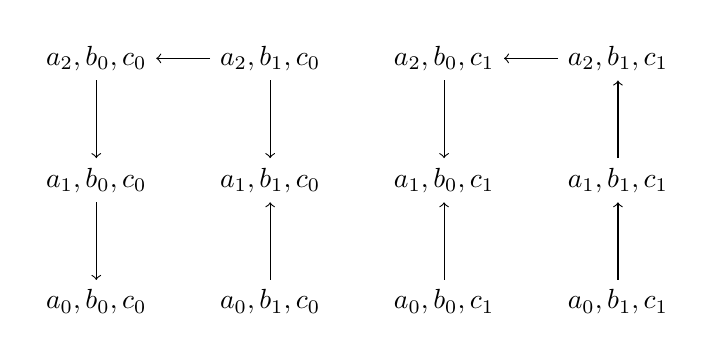
\begin{tikzpicture}
      \matrix [column sep=0.7cm, row sep=1cm]{
        \node (s200) {$\RRBetat{a_2,b_0,c_0}$}; &
        \node (s210) {$\RRBetat{a_2,b_1,c_0}$}; &
        \node (s201) {$\RRBetat{a_2,b_0,c_1}$}; &
        \node (s211) {$\RRBetat{a_2,b_1,c_1}$}; \\
        \node (s100) {$\RRBetat{a_1,b_0,c_0}$}; &
        \node (s110) {$\RRBetat{a_1,b_1,c_0}$}; &
        \node (s101) {$\RRBetat{a_1,b_0,c_1}$}; &
        \node (s111) {$\RRBetat{a_1,b_1,c_1}$}; \\
        \node (s000) {$\RRBetat{a_0,b_0,c_0}$}; &
        \node (s010) {$\RRBetat{a_0,b_1,c_0}$}; &
        \node (s001) {$\RRBetat{a_0,b_0,c_1}$}; &
        \node (s011) {$\RRBetat{a_0,b_1,c_1}$}; \\
      };
      \path[->]
        (s010) edge (s110)
        (s100) edge (s000)
        (s200) edge (s100)
        (s210) edge (s110) edge (s200)
        (s001) edge (s101)
        (s011) edge (s111)
        (s111) edge (s211)
        (s201) edge (s101)
        (s211) edge (s201)
      ;
    \end{tikzpicture}
    \end{center}
    \caption{\figlabel{thomas-dynamique}%
      Représentation de la dynamique du modèle de Thomas donné à la \figref{thomas}.
      Chaque état est représenté par un triplet $\RRBetat{a_i, b_j, c_k}$
      où $i$, $j$ et $k$ représentent respectivement le niveau d'expression de $a$, $b$ et $c$,
      et une transition entre deux états est représentée par une flèche.
    }
  \end{figure}
\end{example}



\subsubsection*{Graphe des interactions minimal}
Il est possible d'inférer le graphe des interactions \emph{minimal} d'un modèle de Thomas,
en ne conservant que les arcs fonctionnels pour la dynamique.
Définissons $f^a(s) = \RRBget{s}{a}$ si $s[a]\in K_{a, \RRBres{a}{s}}$,
et $f^a(s) = \RRBget{s}{a} + \delta^a(s)$ sinon.
Une régulation positive (\resp négative) de $b$ sur $a$ n'est inférée que s'il existe
un état $s$ tel que l'augmentation du niveau de $b$ aurait pour conséquence
une augmentation (\resp diminution) de la valeur de $f^a$ ;
ou, en d'autres termes, s'il existe un état $s$ tel que :
$f^a(s \recouvre b_i) < \text{(\resp $>$) } f^a(s \recouvre b_{i+1})$, 
où $i < l_b$ et $s \recouvre b_i$ est l'état identique à $s$
sauf pour la composante de $b$ qui a été remplacée par $b_i$.
Un tel graphe des interactions peut être utilisé pour inférer des propriétés globales sur
la dynamique \citeaffixed{Richard10,PR11-SASB}{cf. par exemple}.

\subsubsection*{Discussion sur la valeur du plafond}
\label{plafond}
Le plafond $l_a$ d'un composant $a$, qui est le niveau d'expression maximum de $a$,
est généralement choisi comme égal au nombre $\card{\components^+(a)}$
de régulations sortant du nœud $a$ dans le graphe des interactions,
c'est-à-dire le nombre de composants qu'il régule.
En effet, chaque niveau discret dans $\segm{0}{l_a}$ représente un ensemble arbitraire de valeurs
pour une donnée réelle et généralement continue de $a$ (niveau d'activité, concentration, etc.),
et pour laquelle $a$ possède une certaine influence sur plusieurs autres composants qu'il régule.
Ainsi, autoriser des valeurs de $l_a$ plus grandes que $\card{\components^+(a)}$
n'augmente pas l'expressivité du modèle
car plusieurs niveaux d'expression de $a$ auront alors le même rôle au niveau des régulations.
À l'inverse, réduire ce plafond à des valeurs plus petites que $\card{\components^+(a)}$
sous-entendrait que plusieurs seuils de régulations sortant de $a$ sont identiques,
ce qui est biologiquement peu plausible.
Cependant, ces considérations peuvent être ignorées pour des raisons diverses de modélisation,
et nous avons choisi de ne pas contraindre le plafond d'un composant dans ce document
pour des raisons de simplicité.
Ainsi, dans l'exemple de modèle de Thomas de la \figref{thomas},
il serait suffisant d'avoir $l_a = 1$ (et $\arc{a}{-}{1}{b} \in E$)
étant donné que $a$ ne possède qu'une régulation sortante.
La valeur $l_a = 2$ permet cependant de rendre l'exemple plus intéressant
en montrant notamment l'aspect unitaire de la dynamique du modèle de Thomas
(et $\arc{a}{-}{2}{b} \in E$ peut être choisi arbitrairement).

\subsubsection*{Discussion sur les signes}
L'ajout d'arcs non-signés ($\uns$) permet de modéliser des régulations dont la tendance générale
est plus complexe qu'une simple activation ou inhibition.
Il est à noter qu'utiliser $\uns$ comme signe pour étiqueter les régulations en plus
des deux signes habituels $+$ et $-$ n'augmente pas l'expressivité du formalisme.
En effet, les signes n'ont pas d'impact sur la paramétrisation (\defref{thomas-param})
ou sur la dynamique (\defref{thomas-dynamique}).
Ils ont cependant un but informatif, car ils résument les différentes régulations du modèle.
Ils seront d'ailleurs utilisés au \chapref{expressivite}
comme base pour énumérer des paramétrisations incomplètes.
Les arcs non-signés seront de plus exploités pour modéliser un graphe des interactions
avec une connaissance partielle de certaines régulations.
Cependant, comme ils ne sont pas courants dans la littérature,
l'état de l'art de la section suivante portera principalement
sur les modèles de Thomas sans arcs non-signés ($E_\uns = \emptyset$).

%\todo{Hypothèses monotonie / etc.}

\subsubsection*{Discussion sur les intervalles de paramètres}
Tandis que la littérature utilise principalement des paramètres entiers
(c'est-à-dire comportant une unique valeur, par exemple : $K_{a,\omega} = i$)
nous proposons ici d'utiliser des intervalles comme valeurs des paramètres
(par exemple : $K_{a,\omega} = \segm{i}{j}$).
Ces intervalles permettent notamment de faciliter la représentation,
bien qu'il soit intéressant de noter qu'ils augmentent l'expressivité du modèle de Thomas.
En effet, considérons un cas fictif où $K_{a,\omega} = \segm{i}{i+2}$
(c'est-à-dire un intervalle contenant trois valeurs) et $s$ un état tel que
$\RRBres{a}{s} = \omega$.
D'après la \defref{thomas-dynamique}, si $\RRBget{s}{a} \in K_{a,\omega}$, alors $a$
ne peut pas évoluer dans $s$ ; ainsi, $a$ possède trois états locaux stables :
$a_i$, $a_{i+1}$ et $a_{i+2}$.
Ce comportement ne peut pas être retrouvé à l'aide de paramètres entiers,
car il n'est pas possible de distinguer les trois configurations de ressources
correspondant aux trois états locaux.
Au plus deux états stables locaux peuvent être créés à l'aide d'une auto-régulation positive
sur $a$ pour distinguer deux configurations différentes
($\RRBget{s}{a} < t$ et $\RRBget{s}{a} \geq t$)
ce qui n'est cependant pas suffisant pour obtenir trois états stables.



\subsection{Définition des réseaux discrets asynchrones}
\seclabel{rda-def}

Certaines contraintes propres aux modèles de Thomas peuvent être relâchées pour permettre
des comportements supplémentaires.
Ainsi, il est courant de représenter des réseaux de régulation biologique
sous la forme de \emph{réseaux discrets asynchrones}.
Ces réseaux sont aussi fondés sur un graphe des interactions,
mais il utilisent des fonctions d'évolution (\defref{rda-def}) pour plus de permissivité,
en lieu et place de paramètres discrets tels que précédemment
formalisés à la \vdefref{thomas-param}.
Par ailleurs, l'hypothèse d'asynchronisme est conservée car un seul composant peut évoluer
depuis chaque état,
mais leur dynamique n'est pas unitaire dans le cas général
car ce composant peut évoluer d'un nombre arbitraire de niveaux d'expression
(\defref{rda-dynamique}).

\begin{definition}[Réseau discret asynchrone ($\RDA$)]
\deflabel{rda-def}
  Si $\GI = (\components; E)$ est un graphe des interactions,
  un \emph{réseau discret asynchrone} est un couple $\RDA = (\GI; F)$
  avec $F = (f_x)_{x \in \components}$, tels que
  $\forall x \in \components, f_x : \RRBreg{x} \rightarrow \segm{0}{l_x}$.
\end{definition}

\begin{definition}[Dynamique d'un réseau discret asynchrone ($\RRBtransrda{}{}$)]
\deflabel{rda-dynamique}
  Pour tout réseau discret asynchrone $\RDA = (\GI; F)$,
  La dynamique non-unitaire de $\RDA$ est donnée par la relation de transition
  $\RRBtransrda{}{}\ \in \RRBstates \times \RRBstates$ définie par :
  \begin{align*}
    \forall s, s' \in \RRBstates, \RRBtransrda{s}{s'}
      &\Longleftrightarrow \exists a \in \components,
    \RRBget{s}{a} \neq f_a(s) \wedge
      \RRBget{s'}{a} = f_a(s) \\
      &\qquad\quad \wedge \forall b \in \components, b \neq a \Rightarrow \RRBget{s}{b} = \RRBget{s'}{b}
  \end{align*}
\end{definition}

Enfin, nous désignons par \emph{réseau booléen asynchrone}
tout réseau discret asynchrone dont les composants ne possèdent que deux niveaux discrets,
c'est-à-dire tel que : $\forall x \in \components, l_x = 1$.



\subsection{Analyses formelles du modèle de Thomas}
\seclabel{thomas-analyse}

Nous proposons dans cette section un tour d'horizon rapide des différentes méthodes
d'analyse de la dynamique des modèles de Thomas.
Nous nous concentrons principalement sur les méthodes d'analyse statique,
c'est-à-dire permettant d'obtenir des résultats sur la dynamique d'un modèle
sans nécessiter d'en calculer la dynamique de façon complète et explicite.
Ces approches ont l'avantage de jouir d'une faible complexité, même si les résultats formels
qu'elles fournissent sont généralement moins précis ou approximés.
L'analyse du graphe des interactions seul peut ainsi permettre d'obtenir certains
résultats sur sa dynamique,
et la prise en compte de la paramétrisation permet d'affiner cette approche.
Cependant, ces résultats sont insuffisants dans beaucoup de cas,
nécessitant des approches plus exhaustives.
L'analyse complète de la dynamique d'un modèle de Thomas
est généralement invoquée en dernier recours, car elle peut être coûteuse en temps
et en espace mémoire du fait de l'explosion combinatoire inhérente au calcul
de l'espace des états.

\subsubsection*{Analyse du graphe des interactions}
Plusieurs travaux se sont intéressés aux conclusions qui pouvaient être
tirées du seul graphe des interactions.
La recherche d'\emph{états stables}, aussi appelés \emph{points fixes},
présente un intérêt particulier dans l'étude des réseaux de régulation biologique
et a été de fait très étudiée.
Les conjectures de \citefullname{Thomas81}{René}
tracent notamment un lien entre la présence de circuits dans les régulations et celle
d'oscillations ou d'états stables.
Elles se formulent comme suit :
\begin{itemize}
  \item un circuit positif (c.-à-d.~comportant un nombre pair de régulations négatives)
    est une condition nécessaire à la présence de plusieurs points fixes,
  \item un circuit négatif (c.-à-d.~comportant un nombre impair de régulations négatives)
    est une condition nécessaire à la présence d'oscillations soutenues dans la dynamique,
    et donc à la présence d'un attracteur constitué d'au moins deux états.
\end{itemize}
Ces conjectures ont par la suite été démontrées
dans le cas booléen, c'est-à-dire lorsque $\forall x \in \components, l_x = 1$
\cite{RRT08,Richard06thesis}
ainsi que dans le cas multivalué \cite{RiCo07,Richard10}.

Plusieurs résultats viennent de surcroît enrichir ce résultat concernant
l'existence de points fixes.
Des travaux ont par exemple
permis d'obtenir une valeur maximale du nombre de points fixes possibles
dans un modèle de Thomas tant booléen \cite{aracena2008maximum} que multivalué \cite{Richard09}.
Cette valeur dépend du nombre de composants à supprimer pour éliminer
tout circuit positif dans le modèle.
\citeasnoun{PR10-CRAS} ont quant à eux proposé une valeur minimale du nombre de
\emph{points fixes topologiques} d'un modèle booléen.
Ces points fixes ont la particularité de ne pas dépendre de la paramétrisation,
ce qui permet de généraliser un tel résultat à un ensemble de modèles de Thomas.

\subsubsection*{Analyse de la paramétrisation}
Les conditions données précédemment sont \emph{nécessaires} mais non \emph{suffisantes}
pour observer l'apparition des comportements décrits
(oscillations soutenues et multistationnarité).
Plusieurs travaux permettent d'analyser la fonctionnalité des circuits,
c'est-à-dire leur capacité à effectivement «~générer~» ces comportements,
et donc de rendre ces conditions susnommées nécessaires.
Partant d'un modèle de Thomas donné,
il est possible de représenter sa paramétrisation
à l'aide de diagrammes de décision binaires ou multivalués \cite{Bryant86,Srinivasan90}
afin d'en déduire
l'ensemble des états stables mais aussi d'analyser la fonctionnalité des circuits
en effectuant des produits de diagrammes de décision \cite{Naldi07}.
Les différentes façons dont les oscillations soutenues et la multistationnarité
sont «~générées~»
ont aussi été étudiées, ce qui a permis de préciser ces conditions \cite{Comet13}.

% Compression des paramètres : \cite{Naldi07}
%   qui utilisent des BDD : \cite{Bryant86,Srinivasan90}
% Permet certaines analyses efficaces : points fixes et fonctionnalité des circuits

% \subsubsection*{Caractérisation et recherche des points fixes}
% 
% \todo{dispatcher}
% 
% La recherche d'\emph{états stables}, aussi appelés \emph{points fixes},
% présente un intérêt particulier dans l'étude des réseaux de régulation biologique.
% Les conjectures de \citefullname{Thomas81}{René},
% qui ont par la suite été démontrées \cite{RiCo07}
% portent notamment sur ces questions
% en formulant une condition nécessaire à l'existence de plusieurs points fixes.
% Cette condition n'est cependant pas suffisante
% et ne renseigne pas sur le nombre de points fixes.
% %Dans le cadre d'un modèle booléen (tel que $\forall x \in \components, l_x = 1$)
% L'analyse des interactions seules permet de donner une limite supérieure au nombre
% de points fixes \cite{aracena2008maximum,Richard09}
% ainsi que du nombre de points fixes topologiques,
% (c'est-à-dire ne dépendant pas des paramètres) dans le cas booléen
% \cite{PR10-CRAS},
% sans pour autant proposer une énumération exhaustive.
% \citeasnoun{Naldi07} ont proposé une méthode efficace
% basée sur l'utilisation de diagrammes de décision binaires
% pour l'énumération des points fixes.

\subsubsection*{Analyse de la dynamique}
Afin d'obtenir des résultats plus précis sur le comportement d'un modèle,
comme l'activation d'un composant ou la présence d'oscillations sur une partie
donnée du modèle,
ce que les méthodes décrites précédemment ne permettent pas d'obtenir,
il peut devenir nécessaire de faire appel à des techniques
de \textit{model checking} plus poussées
\citeaffixed{Richard06,gallet14adapting}{voir p.~ex.}.
Ces méthodes permettent généralement une analyse exhaustive de la dynamique,
tout en devant faire face à l'explosion combinatoire typique de ce type d'analyse,
qui limite grandement la taille des modèles étudiés.
De telles analyses ont été théorisées par \citeasnoun{bernot04}
et se basent sur l'expression de propriétés exprimées en logiques temporelles
CTL \cite{Clarke82} ou LTL \cite{Pnueli77}.
Elles possèdent l'avantage d'être très complètes
car la dynamique est entièrement explorée et l'expressivité des logiques temporelles permet
d'exprimer beaucoup de propriétés intéressantes,
mais au prix d'une complexité très importante.
Afin de réduire cette complexité,
\citeasnoun{Naldi09} proposent d'effectuer de la réduction de modèles
en éliminant certaine nœuds qui ont un rôle secondaire.
Le modèle obtenu possède une taille inférieure et certaines bonnes propriétés sont conservées,
comme l'ensemble des points fixes et des attracteurs,
au prix d'une dynamique parfois sous-approximée par rapport au modèle d'origine.


% Les Frappes de Processus
\section{Les Frappes de Processus standards}

Cette section définit les Frappes de Processus standards
telles qu'elles ont été formalisées par \citeasnoun{PMR10-TCSB}.
Les Frappes de Processus offrent une représentation discrète, asynchrone et indéterministe
avec une définition atomique des interactions entre les différents composants du modèle.
Elles sont particulièrement adaptées aux représentations des réseaux de régulation biologiques
bien qu'elles soient assez générales pour potentiellement permettre des applications plus
larges en informatique ou dans d'autres domaines.

Nous donnerons tout d'abord à la \secref{ph} une définition des Frappes de Processus standards
%accompagnée d'une discussion,
ainsi qu'un certain nombre de définitions formelles supplémentaires
nécessaires pour la suite de ce manuscrit.
Nous détaillons ensuite à la \secref{sc} le mécanisme particulier des sortes coopératives
tel qu'il avait été formalisé dans les travaux de Loïc Paulevé,
et nous montrerons qu'il permet de représenter l'action conjointe de plusieurs composants,
mais avec certains défauts difficiles à corriger dans cette version du formalisme.
Enfin, nous aborderons brièvement les travaux précédent
concernant l'analyse statique (\secref{ph-as-pf}) qui permet d'obtenir des résultats
sur l'ensemble des états stables ou l'atteignabilité d'un niveau local au sein d'un modèle,
et concernant l'ajout de paramètres stochastiques (\secref{ph-stocha})
dans le but d'introduire une composante temporelle continue dans les Frappes de Processus.



\subsection{Définition}
\seclabel{ph}

Les \emph{Frappes de Processus standards} telles que données à la \defref{ph},
aussi appelées \textit{Process Hitting},
ou plus simplement \emph{Frappes de Processus} dans ce chapitre,
permettent une modélisation atomique et asynchrone des interactions entre composants.
Un modèle de Frappes de Processus standards comporte un nombre fini de \emph{sortes}
généralement notées $a$, $b$, $c$...
Celles-ci permettent de représenter les différentes entités du modèle,
qu'il s'agisse de composant ayant une réalité biologique (gène, protéine...)
ou d'entités nécessaire à la modélisation (comme les sortes coopératives
qui seront décrites à la \secref{sc}).
Chaque sortes contient plusieurs \emph{processus},
qui représentent les différentes
niveaux d'expression discrets accessibles par la sorte,
et qui sont notés $a_i$
où $a$ est le nom de la sorte et $i$ l'indice du processus dans cette sorte.
Un processus n'appartient qu'à une unique sorte.
Chaque processus est dit \emph{actif} s'il représente le niveau d'expression
dans lequel doit se trouver sa sorte à un certain moment.
Un \emph{état} du modèle est donc décrit par l'ensemble des processus actifs à un instant donné,
avec exactement un processus actif par sorte
---~afin de ne pas sur-représenter ou sous-représenter le niveau d'expression courant d'une sorte.

La dynamique est introduite dans les Frappes de Processus par des \emph{actions}
qui permettent de modifier le processus actif d'une sorte,
à la condition éventuelle qu'un processus donné d'une autre sorte soit présent.
Une action consiste donc en un triplet de processus $\PHfrappe{a_i}{b_j}{b_k}$
qui se lit : «~$a_i$ frappe $b_j$ pour le faire bondir en $b_k$~»,
et qui signifie que si, dans un état donné, les processus $a_i$ et $b_j$ sont
tous les deux présents, alors il est possible d'activer $b_k$ (et de désactiver $b_j$)
dans l'état suivant.
Autrement dit, le processus actif de la sorte $b$ peut \emph{bondir}
de $b_j$ à $b_k$ à condition que $a_i$ soit actif ;
lorsque cela arrive, on dit qu'on a \emph{joué} l'action $\PHfrappe{a_i}{b_j}{b_k}$.
Par convention, on contraint de plus que $b_j \neq b_k$ pour assurer que le jeu d'une action
provoque bien un changement de processus actif.
Il est aussi possible de définir une auto-action, où $a_i = b_j$ (et nécessairement $a = b$),
qui permet de représenter le cas particulier où le processus $b_j$ peut bondir en $b_k$
sans autre condition.

Les Frappes de Processus sont conçues comme un formalisme
à temps discret asynchrone, ce qui signifie que
l'évolution d'un tel modèle est modélisée par une succession de pas de temps discrets
qui représentent la succession des états du modèle,
et exactement une action est jouée entre deux états successifs.
Cela implique qu'un seul processus actif à la fois peut bondir entre deux
pas de temps successifs, et donc qu'une seule sorte peut évoluer entre deux états.
De plus, cela rend la dynamique Frappes de Processus indéterministe,
car à tout état du modèle peuvent correspondre plusieurs états successeurs
dans le cas où plusieurs actions peuvent y être jouées.
Enfin, nous notons que si aucune action n'est jouable dans un état, alors celui-ci
ne possède pas de successeurs et le modèle ne peut plus évoluer.

\begin{definition}[Frappes de Processus standards]
\deflabel{ph}
  Les \emph{Frappes de Processus standards} sont définies
  par un triplet $\PH = (\PHs; \PHl; \PHh)$, où :
  \begin{itemize}
    \item $\PHs \DEF \{a, b, \dots\}$ est l'ensemble fini et dénombrable des \emph{sortes} ;
    \item $\PHl \DEF \bigtimes{a \in \PHs} \PHl_a$ est l'ensemble fini des \emph{états},
      où $\PHl_a = \{a_0, \ldots, a_{l_a}\}$ est l'ensemble fini et dénombrable
      des \emph{processus} de la sorte $a \in \PHs$ et $l_a \in \sN^*$.
      Chaque processus appartient à une unique sorte :
      $\forall (a_i; b_j) \in \PHl_a \times \PHl_b, a \neq b \Rightarrow a_i \neq b_j$ ;
    \item $\PHh \DEF \{\PHfrappe{a_i}{b_j}{b_k} \mid (a; b) \in \PHs \times \PHs \wedge
      (a_i; b_j; b_k) \in \PHl_a \times \PHl_b \times \PHl_b \wedge
      b_j \neq b_k \wedge a = b \Rightarrow a_i = b_j \}$ est l'ensemble fini des \emph{actions}.
  \end{itemize}
\end{definition}
%
\noindent
On note $\PHproc \DEF \bigcup_{a \in \PHs} \PHl_a$ l'ensemble de tous les processus.
La sorte d'un processus $a_i$ est donnée par $\PHsort(a_i) = a$ ;
on définit aussi l'ensemble des sortes d'un ensemble de processus par :
$\forall A \subset \Proc, \sortes{A} = \{ \sorte{p} \mid p \in A \}$.
Étant donné un état $s \in \PHl$, le processus de la sorte $a \in \PHs$ présent dans $s$ est donné
par $\PHget{s}{a}$, \cad la coordonnée correspondant à $a$ dans l'état $s$.
Si $a_i \in \PHl_a$, nous définissons la notation : $a_i \in s \EQDEF \PHget{s}{a} = a_i$.
Pour toute action $h = \PHfrappe{a_i}{b_j}{b_k} \in \PHh$,
$a_i$ est appelé le \emph{frappeur}, $b_j$ la \emph{cible} et $b_k$ le \emph{bond} de $h$,
et on note : $\hitter{h} = a_i$, $\target{h} = b_j$ et $\bounce{h} = b_k$.

\begin{example}
\exlabel{metazoan-ph-nocoop}
  La figure \figref{metazoan-ph-nocoop} illustre une représentation possible des
  Frappes de Processus standards.
  Le modèle $\PH = (\PHs, \PHl, \PHh)$ représenté comporte trois sortes :
  $\PHs = \{ a, c, f \}$.
  Chaque sorte comporte exactement deux processus :
  \[\PHl_a = \{ a_0, a_1 \} \enspace;\quad
    \PHl_b = \{ b_0, b_1 \} \enspace;\quad
    \PHl_f = \{ f_0, f_1 \} \enspace.\]
  On peut notamment en déduire le nombre total d'états du système :
  $\card{\PHl} = 2^3 = 8$.
  Enfin, ce modèle comporte 7 actions :
  \begin{align*}
    \PHh = \{\qquad
      \PHfrappe{c_1}{a_1}{a_0}\quad; && \PHfrappe{c_0}{a_0}{a_1}\quad;& \\
      \PHfrappe{c_1}{c_1}{c_0}\quad; && \PHfrappe{f_1}{c_0}{c_1}\quad;& \\
      \PHfrappe{f_1}{a_0}{a_1}\quad; && \PHfrappe{f_0}{c_1}{c_0}\quad;& \\
      \PHfrappe{f_1}{f_1}{f_0}\quad\; &&& 
    \qquad\}
  \end{align*}
  
  Ces Frappes de Processus représentent un modèle simplifié du mécanisme
  de segmentation des métazoaires qui permet par exemple de décrire la production de rayures
  chez les drosophiles.
  Il a été originellement établi \textit{in silico} par \citeasnoun{MSB4100192}
  à l'aide d'un formalisme à base d'équations différentielles,
  et le modèle présenté ici est inspiré du modèle proposé par \citeasnoun{PMR10-TCSB}.
  
  Les trois sortes $a$, $b$ et $c$ de ce modèle représentent différents gènes du système,
  que nous qualifierons d'\emph{actifs} dans le reste de ce document lorsqu'ils seront à l'état 1.
  La production de pigment est déclenchée par le produit du gène $a$,
  et une succession d'activations de celui-ci permet donc de produire des rayures.
  Pour que celles-ci soient régulières, il est donc nécessaire que la durée d'activation
  de $a$ soit constante, et que la durée entre deux activations le soit aussi.
  Ce mécanisme est réglé par le gène $c$ qui inhibe à la fois le gène $a$ à intervalles réguliers,
  et s'inhibe lui-même afin d'avoir le rôle d'une horloge.
  Enfin, le procédé complet est dirigé par le gène $f$ qui, lorsqu'il est actif,
  permet la progression d'un front au niveau duquel les pigments sont déposés.
  Ce gène peut aussi s'auto-inhiber après une certaine période, faisant cesser
  l'oscillation de l'horloge et ainsi la production de rayures.
  
  \begin{figure}[ht]
  \begin{center}
  \scalebox{1.5}{\begin{tikzpicture}
    \TSort{(0,4)}{c}{2}{l}
    \TSort{(1,1)}{f}{2}{l}
    \TSort{(3,4)}{a}{2}{r}
    
    \TAction{c_1}{a_1.west}{a_0.north west}{}{right}
    \TAction{f_1}{c_0.west}{c_1.south west}{bend left=50, in=90}{left}
    \TAction{c_1}{c_1.west}{c_0.north west}{selfhit}{right}
    \TAction{f_1.north east}{f_1.south east}{f_0.north east}%
      {selfhit, min distance=30, bend left, out=150, in=90}{left}
    \TAction{f_0.east}{c_1.south east}{c_0.north east}{bend right=80, in=-120}{left}
    
    % Fausse coopération
    \TAction{f_1.north}{a_0.south west}{a_1.south west}{bend left=20}{left}
    \TAction{c_0}{a_0.west}{a_1.south}{}{left}
    
    \TState{f_1, a_0, c_0}
  \end{tikzpicture}}
  \caption{\figlabel{metazoan-ph-nocoop}%
    Un exemple de Frappes de Processus standards.
    Les sortes sont représentées par des rectangles arrondis 
    contenant des cercles représentant les processus.
    Ainsi, le processus $a_1$ est représenté par le cercle marqué «~1~»
    dans le rectangle étiqueté «~$a$~», etc.
    Chaque action est de plus symbolisée par un couple de flèches,
    l'une en trait plein et l'autre en pointillés ;
    par exemple, l'action $\PHfrappe{c_1}{a_1}{a_0}$
    est représentée par une flèche pleine entre les processus $c_1$ et $a_1$
    suivie d'une flèche en pointillés entre $a_1$ et $a_0$.
    Enfin, les processus grisés représentent un état possible
    pour ces Frappes de Processus : $\etat{a_0, c_0, f_1}$, qui peut aussi faire office
    d'état initial pour ce modèle.
  }
  \end{center}
  \end{figure}
\end{example}

Les séquences d'actions ont un rôle particulier pour les Frappes de Processus.
Elles permettent notamment d'abstraire une dynamique locale en se concentrant
sur la conséquence plutôt que sur la cause,
et seront notamment utiles pour la méthode d'analyse statique développée
au \chapref{phcanonique}.
Pour toute séquence d'actions $A$,
on note $\sortes{A}$ l'ensemble des sortes dont au moins un processus figure dans $A$
en tant que frappeur, cible ou bond d'une action.
De plus, pour toute sorte $a$,
on note $\prem{a}{A}$ le premier processus référencé de $a$,
$\sup{A}$ l'ensemble de tous ces premiers processus,
$\der{a}{A}$ le dernier processus référencé de $a$
et $\fin{A}$ l'ensemble de tous ces derniers processus.
Ces notations sont formellement définies dans la \defref{premder}.

\begin{definition}[$\premsymbol$, $\dersymbol$, $\suppsymbol$ et $\finsymbol$]
\deflabel{premder}
  Pour toute séquence d'actions $A$ et pour toute sorte $a$,
  $\prem{a}{A}$ est le premier processus de $a$ référencé dans $A$,
  en tant que frappeur ou en tant que cible,
  et $\der{a}{A}$ en est le dernier,
  en tant que frappeur ou en tant que bond.
  \begin{align}
  \eqlabel{prem}
    \prem{a}{A} &=
      \begin{cases}
        \varnothing & \text{si } a \notin \sortes{A}, \\
        \hitter{A_m} & \text{si } m = \min\{ n \in \indexes{A} \mid a \in \sortes{A_n} \}
          \wedge \sorte{\hitter{A_m}} = a, \\
        \target{A_m} & \text{sinon si } m = \min\{ n \in \indexes{A} \mid a \in \sortes{A_n} \}
          \wedge \sorte{\target{A_m}} = a \enspace;
      \end{cases} \\
  \eqlabel{der}
    \der{a}{A} &=
      \begin{cases}
        \varnothing & \text{si } a \notin \sorts(A), \\
        \bounce{A_m} & \text{si } m = \max\{ n \in \indexes{A} \mid a \in \sortes{A_n} \}
          \wedge \sorte{\bounce{A_m}} = a, \\
        \hitter{A_m} & \text{sinon si } m = \max\{ n \in \indexes{A} \mid a \in \sortes{A_n} \}
          \wedge \sorte{\hitter{A_m}} = a \enspace.
      \end{cases}
  \end{align}

  Pour toute séquence d'actions $A$,
  $\supp{A}$ et $\fin{A}$ renvoient respectivement à l'ensemble des premiers
  et derniers processus de $A$ pour toutes les sortes qui y figurent.
  \begin{align}
  \eqlabel{supp}
    \supp{A} &= \{ p \in \Proc \mid \sorte{p} \in \sorte{A} \wedge
      p = \prem{\sort{p}}{\delta} \} \enspace, \\
  \eqlabel{fin}
    \fin{A} &= \{ p \in \Proc \mid \sorte{p} \in \sorte{A} \wedge
      p = \der{\sort{p}}{\delta} \} \enspace.
  \end{align}
\end{definition}

La \defref{substate} établit la notion de sous-état sur un ensemble de sortes,
\cad un ensemble de processus qui sont deux à deux de sortes différentes,
ce qui permet de ne considérer qu'une partie d'un état complet.
Nous notons $\PHsubl$ l'ensemble de tous les sous-états et nous constatons qu'un
état est \textit{a fortiori} un sous-état : $\PHl \subset \PHsubl$.
Nous notons de plus $\PHsublset$ l'ensemble des sous-états désordonnés,
c'est-à-dire dont l'ordre entre les sortes a été oublié.
Le recouvrement d'un état $s$ par un processus $a_i$ est formalisé à la \defref{statecap}
par un état identique à $s$, sauf pour le processus de $a$ qui a été remplacé par $a_i$,
ce qui permettra de définir la dynamique des Frappes de Processus %avec $k$ classes de priorités
à la \defref{play}.
La définition de recouvrement est aussi étendue à un sous-état désordonné,
autrement dit, à un ensemble de processus contenant au plus un processus par sorte.

\begin{definition}[Sous-états ($\PHsublize{\PHl}$)]
\deflabel{substate}
  Si $S \subset \PHs$ est un ensemble de sortes, un sous-état sur $S$ est un élément de :
  $\PHsubl[\PHl]_S \DEF \bigtimes{a \in S} \PHl_a$.
  L'ensemble de tous les sous-états est noté :
  $\PHsubl[\PHl] \DEF \bigcup_{S \in\powerset(\PHs)} \PHsubl[\PHl]_S$.
  
  \noindent
  De plus, si $\mysigma \in \PHsubl[\PHl]$ et $s \in \PHl$, on note alors :
  \[\mysigma \subseteq s \EQDEF \forall a_i \in \Proc, a_i \in \mysigma \Rightarrow a_i \in s
    \enspace.\]
  
  \noindent
  Enfin, si $S \subset \PHs$, on note :
  $\PHsublset_S = \{ \toset{ps} \subset \Proc \mid ps \in \PHsubl_S \}$
  et
  $\PHsublset = \{ \toset{ps} \subset \Proc \mid ps \in \PHsubl \}$.
\end{definition}
%
\begin{definition}[Recouvrement ($\recouvre : \PHl \times \PHproc \rightarrow \PHl$)]
\deflabel{statecap}
  Étant donné un état $s \in \PHl$ et un processus $a_i \in \PHproc$,
  $(s \recouvre a_i)$ est l'état défini par :
  $\PHget{(s \recouvre a_i)}{a} = a_i \wedge \forall b \neq a, \PHget{(s \recouvre a_i)}{b} = \PHget{s}{b}$.
  On étend de plus cette définition à un ensemble de processus
  par le recouvrement de l'état par chaque processus,
  à condition que les processus de l'ensemble soient tous de sortes différentes :
  $\forall ps \in \PHsublset, s \recouvre ps = s \underset{a_i \in ps}{\recouvre} a_i$.
\end{definition}

Une propriété de jouabilité telle que décrite à la \defref{ppl}
est équivalente à une formule booléenne dont les atomes sont des processus dans $\Proc$.
Le langage des propriétés de jouabilité permet de décrire la présence d'une configuration
de processus actifs dans un état donné.
Il permet notamment de décrire en termes formels la jouabilité d'une action,
ce qui est immédiatement mis en pratique dans la \defref{fopph}.

\begin{definition}[Propriété de jouabilité ($\F$)]
  \label{def:ppl}
  Une \emph{propriété de jouabilité} est un élément du langage $\F$ défini \todo{inductivement ?} par :
  \begin{itemize}
    \item $\top$ et $\bot$ appartiennent à $\F$ ;
    \item si $a \in \PHs$ et $a_i \in \PHl_a$, alors $a_i$ appartient à $\F$
      et est appelé un \emph{atome} ;
    \item si $P \in \F$ et $Q \in \F$,
      alors $\neg P$, $P \wedge Q$ et $P \vee Q$ appartiennent à $\F$.
  \end{itemize}
%
  Si $P \in \F$ est une propriété de jouabilité et $\mysigma \in \PHsubl$ est un sous-état,
  on note $\Feval{P}{\mysigma}$ l'\emph{évaluation} de $P$ dans $\mysigma$:
  \begin{itemize}
    \item si $P = a_i \in \PHl_a$ est un atome, avec $a \in \PHs$,
      alors $\Feval{a_i}{\mysigma}$ est vraie si et seulement si $a_i \in \mysigma$ ;
    \item si $P$ n'est pas un atome, alors $\Feval{P}{\mysigma}$ est vraie si et seulement si
      on peut l'évaluer récursivement comme vraie en utilisant la sémantique habituelle des
      opérateurs $\neg$, $\wedge$ et $\vee$ et des constantes $\top$ et $\bot$.
  \end{itemize}
%
  Une fonction $\Fopsymbol : \PHh \rightarrow \F$ associant à toute action une propriété de jouabilité
  est appelée un \emph{opérateur de jouabilité}.
\end{definition}

Étant donné que ce langage n'utilise que des opérateur logiques classiques,
les propriétés de la logique booléenne sont applicables aux propriétés de jouabilité,
à savoir celles concernant la distributivité, l'associativité et la commutativité,
ainsi que les lois de De Morgan concernant la négation.

Il en résulte notamment la propriété suivante, permettant d'évaluer la négation d'un atome,
et qui dérive naturellement du fait que si un processus n'est pas actif dans un état donné,
cela signifie alors qu'un autre processus de la même sorte l'est :
\[\forall a \in \PHs, \forall a_i \in \PHl_a, \forall \mysigma \in \PHsubl,
  \Feval{\neg a_i}{\mysigma} \Leftrightarrow
  \Feval{\bigvee_{\substack{a_j \in \PHl_a\\a_j \neq a_i}} a_j}{\mysigma}\]

Enfin, on note dans la suite :
\[\forall A \in \PHsublset, \Fconj{A} \equiv \bigwedge_{p \in A} p \enspace.\]

\todo{Gluer}

\begin{definition}[Opérateur de jouabilité ($\Fopsymbol : \PHh \rightarrow \F$)]
\deflabel{fopph}
  L'opérateur de jouabilité des Frappes de Processus est défini par :
  \[\forall h \in \PHh, \Fop{h} \equiv \hitter{h} \wedge \target{h} \enspace.\]
\end{definition}

\begin{definition}[Dynamique des Frappes de Processus ($\PHtrans$)]
\deflabel{play}
  Une action $h \in \PHh$ est dite \emph{jouable}
  dans l'état $s \in \PHl$ si et seulement si :
  $\Feval{\Fop{h}}{s}$.
%  $\target{h} \in s \wedge \Feval{\Fop{h}}{s}$.
  Dans ce cas, $(s \PHplay h)$ est l'état résultant du jeu de l'action $h$ dans $s$,
  et on le définit par : $(s \PHplay h) = s \recouvre \bounce{h}$.
  De plus, on note alors : $s \PHtrans (s \PHplay h)$.

  Si $s \in \PHl$, un \emph{scénario} $\delta$ dans $s$
  est une séquence d'actions de $\PHh$ qui peuvent être jouées successivement dans $s$.
  L'ensemble de tous les scénarios dans $s$ est noté $\Sce(s)$.
\end{definition}

\begin{example}
  La séquence d'actions suivantes est un scénario dans l'état \TODO des Frappes de Processus
  de la \figref{metazoan-ph-nocoop} :
  \TODO
\end{example}



\subsection{Sortes coopératives}
\seclabel{sc}

\TODO


\todo{Figure d'exemple de sorte coopérative}

\begin{example}
\exlabel{metazoan-ph}
  Le modèle de Frappes de Processus de la \figref{metazoan-ph-nocoop}
  représentant le mécanisme de segmentation métazoaire évoqué à la page
  \expageref{metazoan-ph-nocoop},
  la production de pigment devrait uniquement être possible à la condition suivante :
  «~$f$ est actif et $c$ n'est pas actif~».
  Or dans l'état courant du modèle,
  la désactivation du gène $f$ n'empêche pas la production de pigment,
  car depuis tout état contenant $f_0$, il est toujours possible d'activer $a$
  à l'aide des actions $\PHfrappe{f_0}{c_1}{c_0}$ et $\PHfrappe{c_0}{a_0}{a_1}$.
  
  Afin de pallier partiellement ce défaut, il est possible d'ajouter une sorte coopérative $fc$,
  comme à la \figref{metazoan-ph},
  afin de détecter la présence de $f_1$ et $c_0$.
  Les deux actions $\PHfrappe{c_0}{a_0}{a_1}$ et $\PHfrappe{c_0}{a_0}{a_1}$
  sont alors remplacées par une action $\PHfrappe{fc_{10}}{a_0}{a_1}$
  afin d'avoir une véritable coopération entre ces deux processus pour activer $a$.
  
  \begin{figure}[ht]
  \begin{center}
  \begin{tikzpicture}
    \TSort{(0,4)}{c}{2}{l}
    \TSort{(1,0)}{f}{2}{l}
    \TSort{(7,4)}{a}{2}{r}
    
    \TSetTick{fc}{0}{00}
    \TSetTick{fc}{1}{01}
    \TSetTick{fc}{2}{10}
    \TSetTick{fc}{3}{11}
    \TSort{(4,1)}{fc}{4}{r}
    
    \TAction{fc_2}{a_0.west}{a_1.south west}{}{left}
    \TAction{c_1}{a_1.west}{a_0.north west}{}{right}
    \TAction{f_1}{c_0.west}{c_1.south west}{bend left=30, in=90}{left}
    \TAction{c_1}{c_1.west}{c_0.north west}{selfhit}{right}
    \TAction{f_1.north east}{f_1.south east}{f_0.north east}%
      {selfhit, min distance=30, bend left, out=150, in=90}{left}
    \TAction{f_0.east}{c_1.south east}{c_0.north east}{bend right=60, in=-140}{left}
    
    \path (1.8, 0.5) edge[coopupdate] (3.2, 2);
    \path (0.8, 4.5) edge[coopupdate] (3.2, 3);
    
    \TState{f_1, a_0, c_0, fc_2}
  \end{tikzpicture}
  \caption{\figlabel{metazoan-ph}%
    Amélioration du modèle de Frappes de Processus de la \figref{metazoan-ph-nocoop}
    à l'aide de la sorte coopérative $fc$.
    Les processus de cette sorte représentent les différents sous-états formés par les
    deux sortes $f$ et $c$.
    Ainsi, $fc_{00}$ représente le fait que $f_0$ et $c_0$ sont actifs, etc.
    Les actions permettant la mise à jour de cette sorte coopérative n'ont pas
    été représentée explicitement mais sont symbolisées par les deux flèches
    en zigzag provenant de $f$ et $c$.
  }
  \end{center}
  \end{figure}
\end{example}

\todo{Explications sur l'imperfection des sortes coopératives}

\begin{example}
  Malgré l'ajout d'une sorte coopérative $fc$ dans le modèle
  de la \figref{metazoan-ph-nocoop},
  il faut noter que le comportement désiré n'est pas exactement atteint.
  En effet, l'ajout de cette sorte coopérative devait permettre d'éviter toute activation de $a$
  lorsque $f$ devenait inactif, en permettant par exemple de jouer ce type de scénario
  depuis l'état initial $\etat{a_0, c_0, f_1, fc_{10}}$ :
    \[\PHfrappe{f_1}{f_1}{f_0} \cons \PHfrappe{f_0}{fc_{10}}{fc_{00}}\]
  après lequel il n'est plus possible d'atteindre un état où $a_1$ est actif.
  
  Cependant, il se trouve qu'il existe encore un cas particulier où $a$ peut être activé
  malgré la présence de $f_0$.
  Ce cas particulier relève du comportement mis en valeur \todo{dans les paragraphes ci-dessus},
  où une action a pour frappeur un processus de sorte coopératif qui ne devrait pas être
  actif si celle-ci avait été mise à jour.
  Il s'observe par exemple en jouant le scénario suivant depuis l'état initial
  $\etat{a_0, c_0, f_1, fc_{10}}$ :
    \[\PHfrappe{f_1}{f_1}{f_0} \cons \PHfrappe{fc_{10}}{a_0}{a_1} \enspace,\]
  ce qui est possible parce que la sorte $fc$ n'a pas été mise à jour avant le jeu
  de l'action $\PHfrappe{fc_{10}}{a_0}{a_1}$.
\end{example}

\begin{comment}
\subsection{Modelling cooperation}
\label{ssec:cooperation}

Cooperation between processes to make another process bounce can be expressed in PH by building a \emph{cooperative sort}, as described in \cite{PMR10-TCSB}.
\pref{fig:ph-livelock} shows an example of cooperation between processes $a_1$ and $b_1$ to make $c_0$ bounce to $c_1$:
a cooperative sort $ab$ is defined with 4 processes (one for each sub-state of the presence of processes $a_1$ and $b_1$).
For the sake of clarity, the processes of $ab$ are indexed using the sub-state they represent.
Hence, $ab_{10}$ represents the sub-state $\PHstate{a_1,b_0}$, and so on.
Each process of sort $a$ and $b$ hit $ab$ to make it bounce to the process reflecting the status of the sorts $a$ and $b$
(\eg $\PHfrappe{a_1}{ab_{00}}{ab_{10}}$ and $\PHfrappe{a_1}{ab_{01}}{ab_{11}}$).
Then, to represent the cooperation between $a_1$ and $b_1$, the process $ab_{11}$ hits $c_0$ to make it bounce to $c_1$ instead of independent hits from $a_1$ and $b_1$.

We note that cooperative sorts are standard PH sorts and do not involve any
special treatment regarding the semantics of related actions.
Furthermore, it is possible to “factorise” cooperative sorts in order to decrease the number of processes created within each cooperative sort.
For example, if three processes $x_1$, $y_1$ and $z_1$ cooperate,
it is preferable to create a cooperative sort $xy$ with 4 processes to state the presence of $x_1$ and $y_1$
and a second cooperative sort $xyz$ with 4 processes to state the presence of $xy_{11}$ and $z_1$,
rather than a unique cooperative sort with 8 processes stating the presence of $x_1$, $y_1$ and $z_1$.
This “factorisation” allows to prevent the combinatorial explosion of the number of processes in cooperative sorts,
especially for cooperations between more than three processes.
It may have computational consequences as the static analysis method developed in~\pref{sec:sa} does not suffer from the number of sorts but from the number of processes in each sort.

The construction of cooperation in PH allows to encode any Boolean function between cooperating processes \cite{PMR10-TCSB}.
Due to the introduction of priorities into the PH framework,
it is possible to build cooperations with no temporal shift by defining actions updating the cooperative sorts with the highest class of priority.
This allows to gain the same expressivity in PH than in Boolean networks, as stated in \pref{sec:dn}.
The aim of this paper is to allow the static analysis of the dynamics to be handled on PH models involving such prioritised actions updating cooperative sorts.
\end{comment}



\subsection{Analyse statique}
\seclabel{ph-as-pf}

\todo{Rappels sur les résultats d'analyse statique (cf. MSCS'10)}

\todo{+ Points fixes}



\subsection{Analyse stochastique}
\seclabel{ph-stocha}

\todo{Rappels rapides ?}

